The QR Layer consists of two primary subsytems: the Scanner and PLC interface. This layer is responsible for scanning the QR codes on each box, retrieving the relevant data (box size, weight, center position) and transmitting the data to the PLC for further processing.

\begin{figure}[h!]
	\centering
 	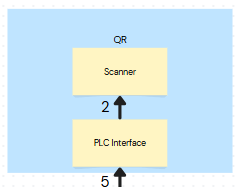
\includegraphics[width=0.60\textwidth]{images/Qr}
 \caption{Example subsystem description diagram}
\end{figure}


\subsection{Scanner}
The scanner subsystem is responsible for reading the QR codes on boxes as they enter the field of view of the camera. The QR codes will be positioned in the center of each box strategicall so as to be able to extract the data related to the box's dimesinons and position. The data is then forwarded to the PLC interface for processing byb the PLC.
\subsubsection{Assumptions}
The assumption is that all boxes on the conveyor belt will have QR codes correctly positioned and free from any obstructions. The scanner will only scan one box at a time and have ample time process the information, as well as re-process if there are any miss readings or missing information from the QR code.

\subsubsection{Responsibilities}
The sole responsibilty of the scanner is to read the QR codes on the boxes, parsing essential box dat into a format that is compatible with the PLC interface. Data is only transmitted when a successful scan is achieved.

\subsubsection{Subsystem Interfaces}

\begin {table}[H]
\caption {Scanner Subsystem interface} 
\begin{center}
    \begin{tabular}{ | p{1cm} | p{6cm} | p{3cm} | p{3cm} |}
    \hline
    ID & Description & Inputs & Outputs \\ \hline
    \#14 & QR code interface & \pbox{3cm}{QR code } & \pbox{3cm}{Parsed box data}  \\ \hline
    \end{tabular}
\end{center}
\end{table}

\subsection{PLC Interface Subsystem}
The PLC interface subsystem acts as a bridge between the scanner and the PLC. After receiving the parsed box data from the scanner, it formats and transmits this information to the PLC's input function. This subsystem esnures that the data is correctly structed for further processing in the PLC, allowing the system to execute appropriate palletizing commands based on the box dimesnions.
\subsubsection{Assumptions}
The data from the scanner is received in a standardized format, requiring minimal processing before it reaches the PLC. The PLC interface does not need to handle multiple data streams simultaneously, as each box is processed sequentially.

\subsubsection{Responsibilities}
The responsibility of the PLC interface subsystem is to format the data as required by the PLC's input function, and esnure smooth communication between the scanner and PLC systems.

\subsubsection{Subsystem Interfaces}

\begin {table}[H]
\caption {Scanner Subsystem interface} 
\begin{center}
    \begin{tabular}{ | p{1cm} | p{6cm} | p{3cm} | p{3cm} |}
    \hline
    ID & Description & Inputs & Outputs \\ \hline
    \#15 & Data transfer for PLC & \pbox{3cm}{Parsed box data from Scanner} & \pbox{3cm}{Formatted data for PLC Input function}  \\ \hline
    \end{tabular}
\end{center}
\end{table}


